\section{问题四：极端油价风险与自适应调价规则}

\subsection{条件尾部分布：FHS--GJR--GARCH}

前三问研究已实现冲击，问题四进一步回答：在2026年6月30日信息集下，未来油价
进入历史高位区间的条件概率多大，以及国内调价机制应如何随压力状态变化。令日收益率
$r_t=\mu+\varepsilon_t$，条件方差服从式\eqref{eq:gjr}。先估计GJR--GARCH，再将
标准化残差 $z_t=\varepsilon_t/\sqrt{h_t}$ 从截止日前经验分布有放回抽样，递归生成

\begin{equation}
  P_{t+k}^{(b)}=P_{t+k-1}^{(b)}
  \exp\!\left(\mu+\sqrt{h_{t+k}^{(b)}}z_{t+k}^{(b)}\right).
  \label{eq:fhs}
\end{equation}

每个期限模拟20000条路径。基线为恒定均值、恒定波动的高斯随机游走，并与主方法使用
相同滚动原点、期限和评价口径。历史90\% 与95\% 价格分位分别为111.397和
115.550美元/桶，只作为上行压力阈值，不作为未来必达价格。

\begin{figure}[H]
  \centering
  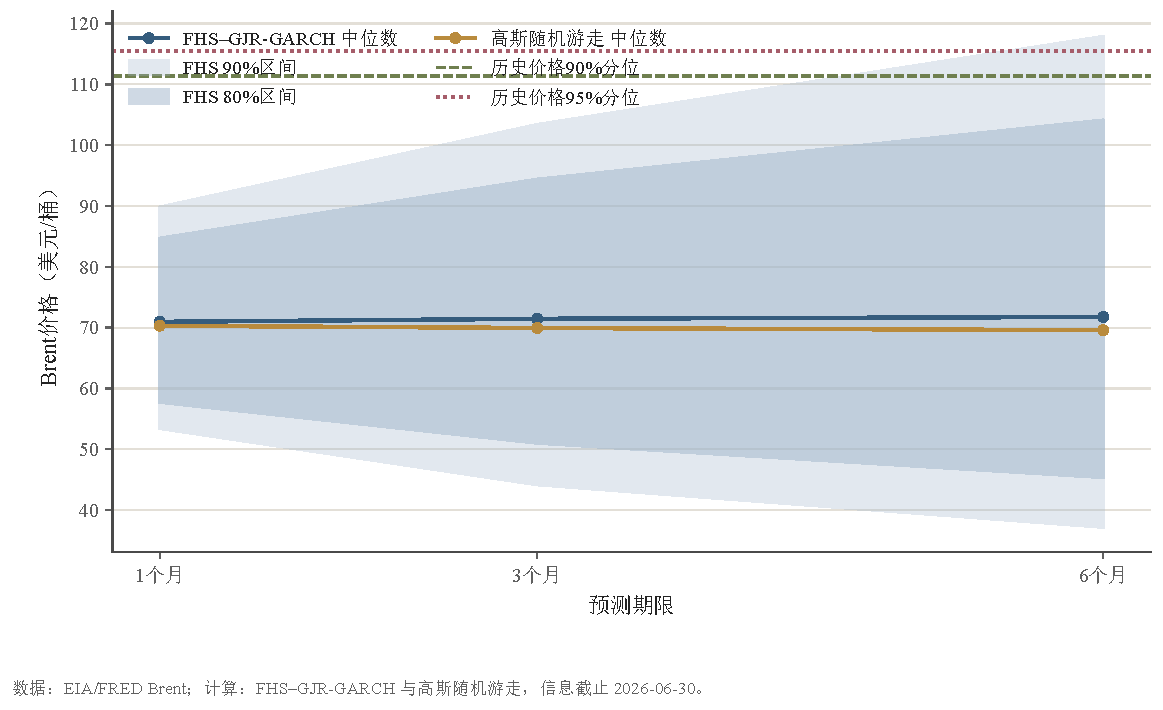
\includegraphics[width=0.91\textwidth]{../figures/q4_price_tail_risk.pdf}
  \caption{固定截止日下Brent条件尾部分布与历史高位阈值}
  \label{fig:q4-tail}
\end{figure}

\begin{table}[H]
  \centering
  \small
  \caption{FHS--GJR--GARCH的油价条件风险预测}
  \label{tab:q4-tail}
  \begin{tabular}{ccccc}
    \toprule
    期限/月 & 中位数 & 90\% 区间 & 期末超过历史95\% 阈值 & 路径内曾越过 \\
    \midrule
    1 & 70.95 & $[53.41,\,89.82]$ & 0.27\% & 0.37\% \\
    3 & 71.46 & $[44.15,\,103.41]$ & 2.27\% & 3.76\% \\
    6 & 71.76 & $[37.15,\,117.90]$ & 5.56\% & 9.65\% \\
    \bottomrule
  \end{tabular}
\end{table}

随着期限延长，中位数仍约为71美元/桶，但分布显著展开，六个月路径内越过历史95\%
阈值的条件概率达到9.65\%。15个季度末原点的统一回测显示：FHS与高斯基线在1、3、
6月的平均分位损失分别为1.639对1.624、2.303对2.483、3.888对3.814。
主方法只在三月期损失更低，而其90\% 区间平均宽度在三个期限均较窄。因此，FHS的
价值主要在于刻画条件异方差和非对称尾部，并非所有期限都全面胜过简单基线。

\subsection{结构冲击宏观压力与已实现政策缓冲}

为避免把模拟价格机械转换为结构冲击，宏观压力直接使用问题一石油特定风险冲击的历史
正向75\%、90\%、95\% 分位数 $s_q$，按

\begin{equation}
  \Delta y_h(s_q)=s_q\widehat\theta_{y,h}
  \label{eq:macrostress}
\end{equation}

缩放问题二响应及联合置信区间。95\% 分位冲击值为1.471。其6月和12月条件响应中，
PPI为0.875、0.493个百分点，CPI为0.267、0.240个百分点，IAV为 $-0.435$、
$-0.628$ 个百分点；六项联合95\% 区间均跨零，故只作为条件压力情景。

政策压力层不把上述情景与问题三反事实相加，而只重述已实现2026路径：相对关闭临时
调控，实际政策截至6月避免的PPI、CPI上行分别为3.370和0.819个百分点，避免的
IAV损失为2.093个百分点。前者来自历史结构冲击的条件响应，后者来自已实现政策路径的
局部反事实，二者识别层级不同。

\subsection{SAPR--CVaR三状态调价规则}

固定传导率难以同时兼顾日常价格信号和极端期宏观稳定。本文在现行机制应调额
$A_t^{rule}$ 上增加状态自适应平滑层。用开发样本中正向机制应调额的75\% 和95\%
分位确定压力阈值435.973和702.491元/吨，并将月份划分为普通、压力和极端状态。
设相应传导率为 $\rho_N\ge\rho_S\ge\rho_E$。若上期仍有未调价差额 $G_{t-1}$，则

\begin{align}
  D_t &= A_t^{rule}+G_{t-1}, \\
  A_t^{SAPR} &=
  \begin{cases}
    \rho_{g_t}D_t, & D_t>0,\\
    D_t, & D_t\le 0,
  \end{cases} \\
  G_t &=
  \begin{cases}
    D_t-A_t^{SAPR}, & D_t>0,\\
    0, & D_t\le 0.
  \end{cases}
  \label{eq:sapr}
\end{align}

这里的负向应调额优先冲销延期差额，避免缺口无限积累。以2026年6月官方价格
9504元/吨为统一基价，将调价收益输入由问题三估计的PPI、CPI、IAV动态核。对每条
六个月情景计算标准化月度宏观损失

\begin{equation}
  L_s=\frac{1}{6}\sum_{t=1}^{6}\left[
  \frac{\max(PPI_{s,t},0)}{\sigma_{PPI}}+
  \frac{\max(CPI_{s,t},0)}{\sigma_{CPI}}+
  \frac{\max(-IAV_{s,t},0)}{\sigma_{IAV}}\right].
  \label{eq:macroloss}
\end{equation}

四个同时最小化的目标为

\begin{equation}
  J_1=\mathbb E(L_s),\quad
  J_2=CVaR_{0.95}(L_s),\quad
  J_3=\mathbb E\!\left[\frac{\sum_{t=1}^{6}G_{s,t}+G_{s,6}}{9504}\right],\quad
  J_4=SD(\Delta\ln F_{s,t}).
  \label{eq:objectives}
\end{equation}

传导率在 $\{0,0.05,\ldots,1\}$ 上枚举，并施加单调约束，共得到1771条规则。只使用
2013年3月至2021年12月的101个六个月开发情景选阈值和规则；2022年1月至
2026年6月的49个情景完全隔离用于检验。对四目标做Pareto支配筛选后保留855条
规则，再将各目标在Pareto集内归一化，选择到理想点欧氏距离最小的唯一膝点。

\begin{figure}[H]
  \centering
  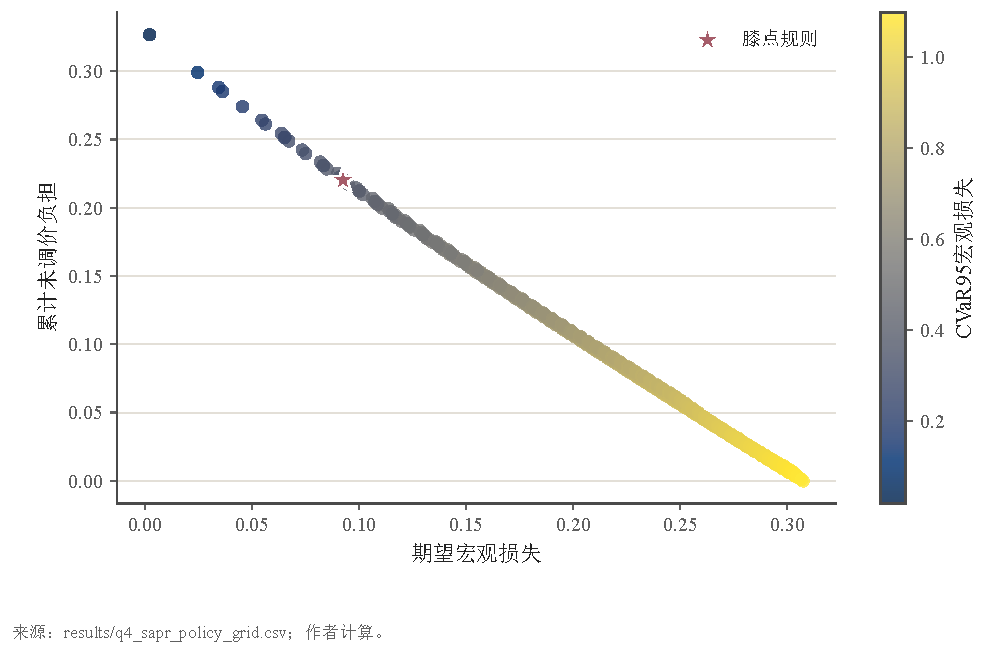
\includegraphics[width=0.88\textwidth]{../figures/q4_sapr_pareto_front.pdf}
  \caption{SAPR--CVaR四目标Pareto前沿与膝点规则}
  \label{fig:q4-pareto}
\end{figure}

膝点规则及其开发样本四目标分别为
\begin{equation}
  (\rho_N,\rho_S,\rho_E)=(0.20,0.05,0.05),
  \label{eq:sapr-knee}
\end{equation}
\begin{equation}
  (J_1,J_2,J_3,J_4)=(0.0925,0.3733,0.2201,0.0317).
  \label{eq:sapr-dev-objectives}
\end{equation}
隔离检验结果见表\ref{tab:q4-sapr}和图\ref{fig:q4-strategy}。

\begin{table}[H]
  \centering
  \small
  \caption{隔离检验样本的调价策略比较}
  \label{tab:q4-sapr}
  \begin{tabularx}{0.97\textwidth}{Xcccc}
    \toprule
    策略 & 平均宏观损失 $J_1$ & 95\% CVaR $J_2$ & 延期负担 $J_3$ & 调价波动 $J_4$ \\
    \midrule
    SAPR膝点 & 0.0908 & 0.5580 & 0.2394 & 0.0255 \\
    完全传导 & 0.3155 & 1.9571 & 0 & 0.0503 \\
    2026临时调控近似 & 0.2941 & 1.7681 & 0.0221 & 0.0426 \\
    统一75\% 平滑 & 0.2812 & 1.7916 & 0.0370 & 0.0438 \\
    \bottomrule
  \end{tabularx}
\end{table}

\begin{figure}[H]
  \centering
  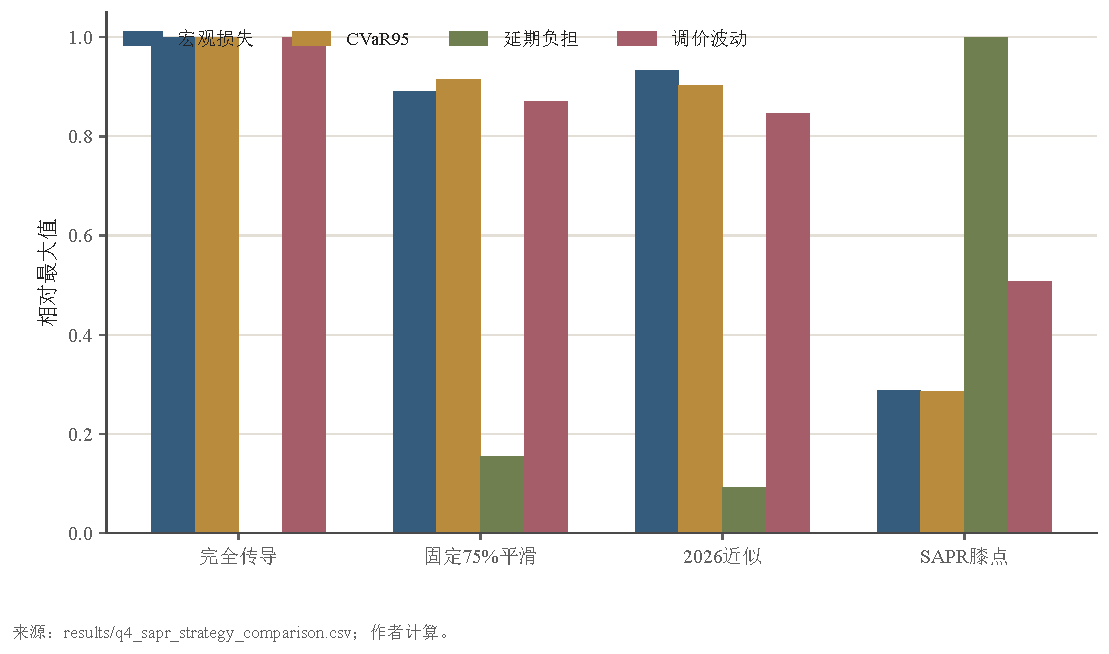
\includegraphics[width=0.90\textwidth]{../figures/q4_sapr_strategy_comparison.pdf}
  \caption{隔离检验样本中四类调价策略的多目标比较}
  \label{fig:q4-strategy}
\end{figure}

SAPR在检验样本的平均和尾部宏观损失、调价波动均低于三类预注册基线，但以较高延期
负担为代价。2000次参数抽样和块bootstrap中，SAPR保持不被基线支配的比例为1.000；
这表示模型参数不确定性下的相对稳定性，不是现实政策成功概率。2026实际冲击情景中，
SAPR、实际政策路径与完全传导的宏观损失分别为0.794、1.648和2.413，但SAPR延期
负担比例达到1.444，明显高于实际路径0.710。这一权衡说明极端期可以强化平滑，却必须
配套透明的缺口上限与退出机制。

\subsection{问题四小结}

固定截止日下，未来六个月Brent期末超过历史95\% 高位的条件概率为5.56\%，路径内
曾越过的概率为9.65\%；这些是风险分布而非确定预测。SAPR--CVaR在注册规则族内给出
普通期20\%、压力与极端期5\% 的膝点传导率，并在隔离检验中保持非支配，但延期负担
不可忽略。因此，建议把状态自适应平滑理解为临时风险管理层，而非替代现行定价机制的
无成本全局最优政策。
